\section{Let's the fun begin!}
\newthought{We are left to define derivatives} of functions between manifolds.
And, since we saw that euclidean spaces are manifolds, we better find a definition that coincides with the one you saw in your analysis courses.

\begin{marginfigure}[7em]
  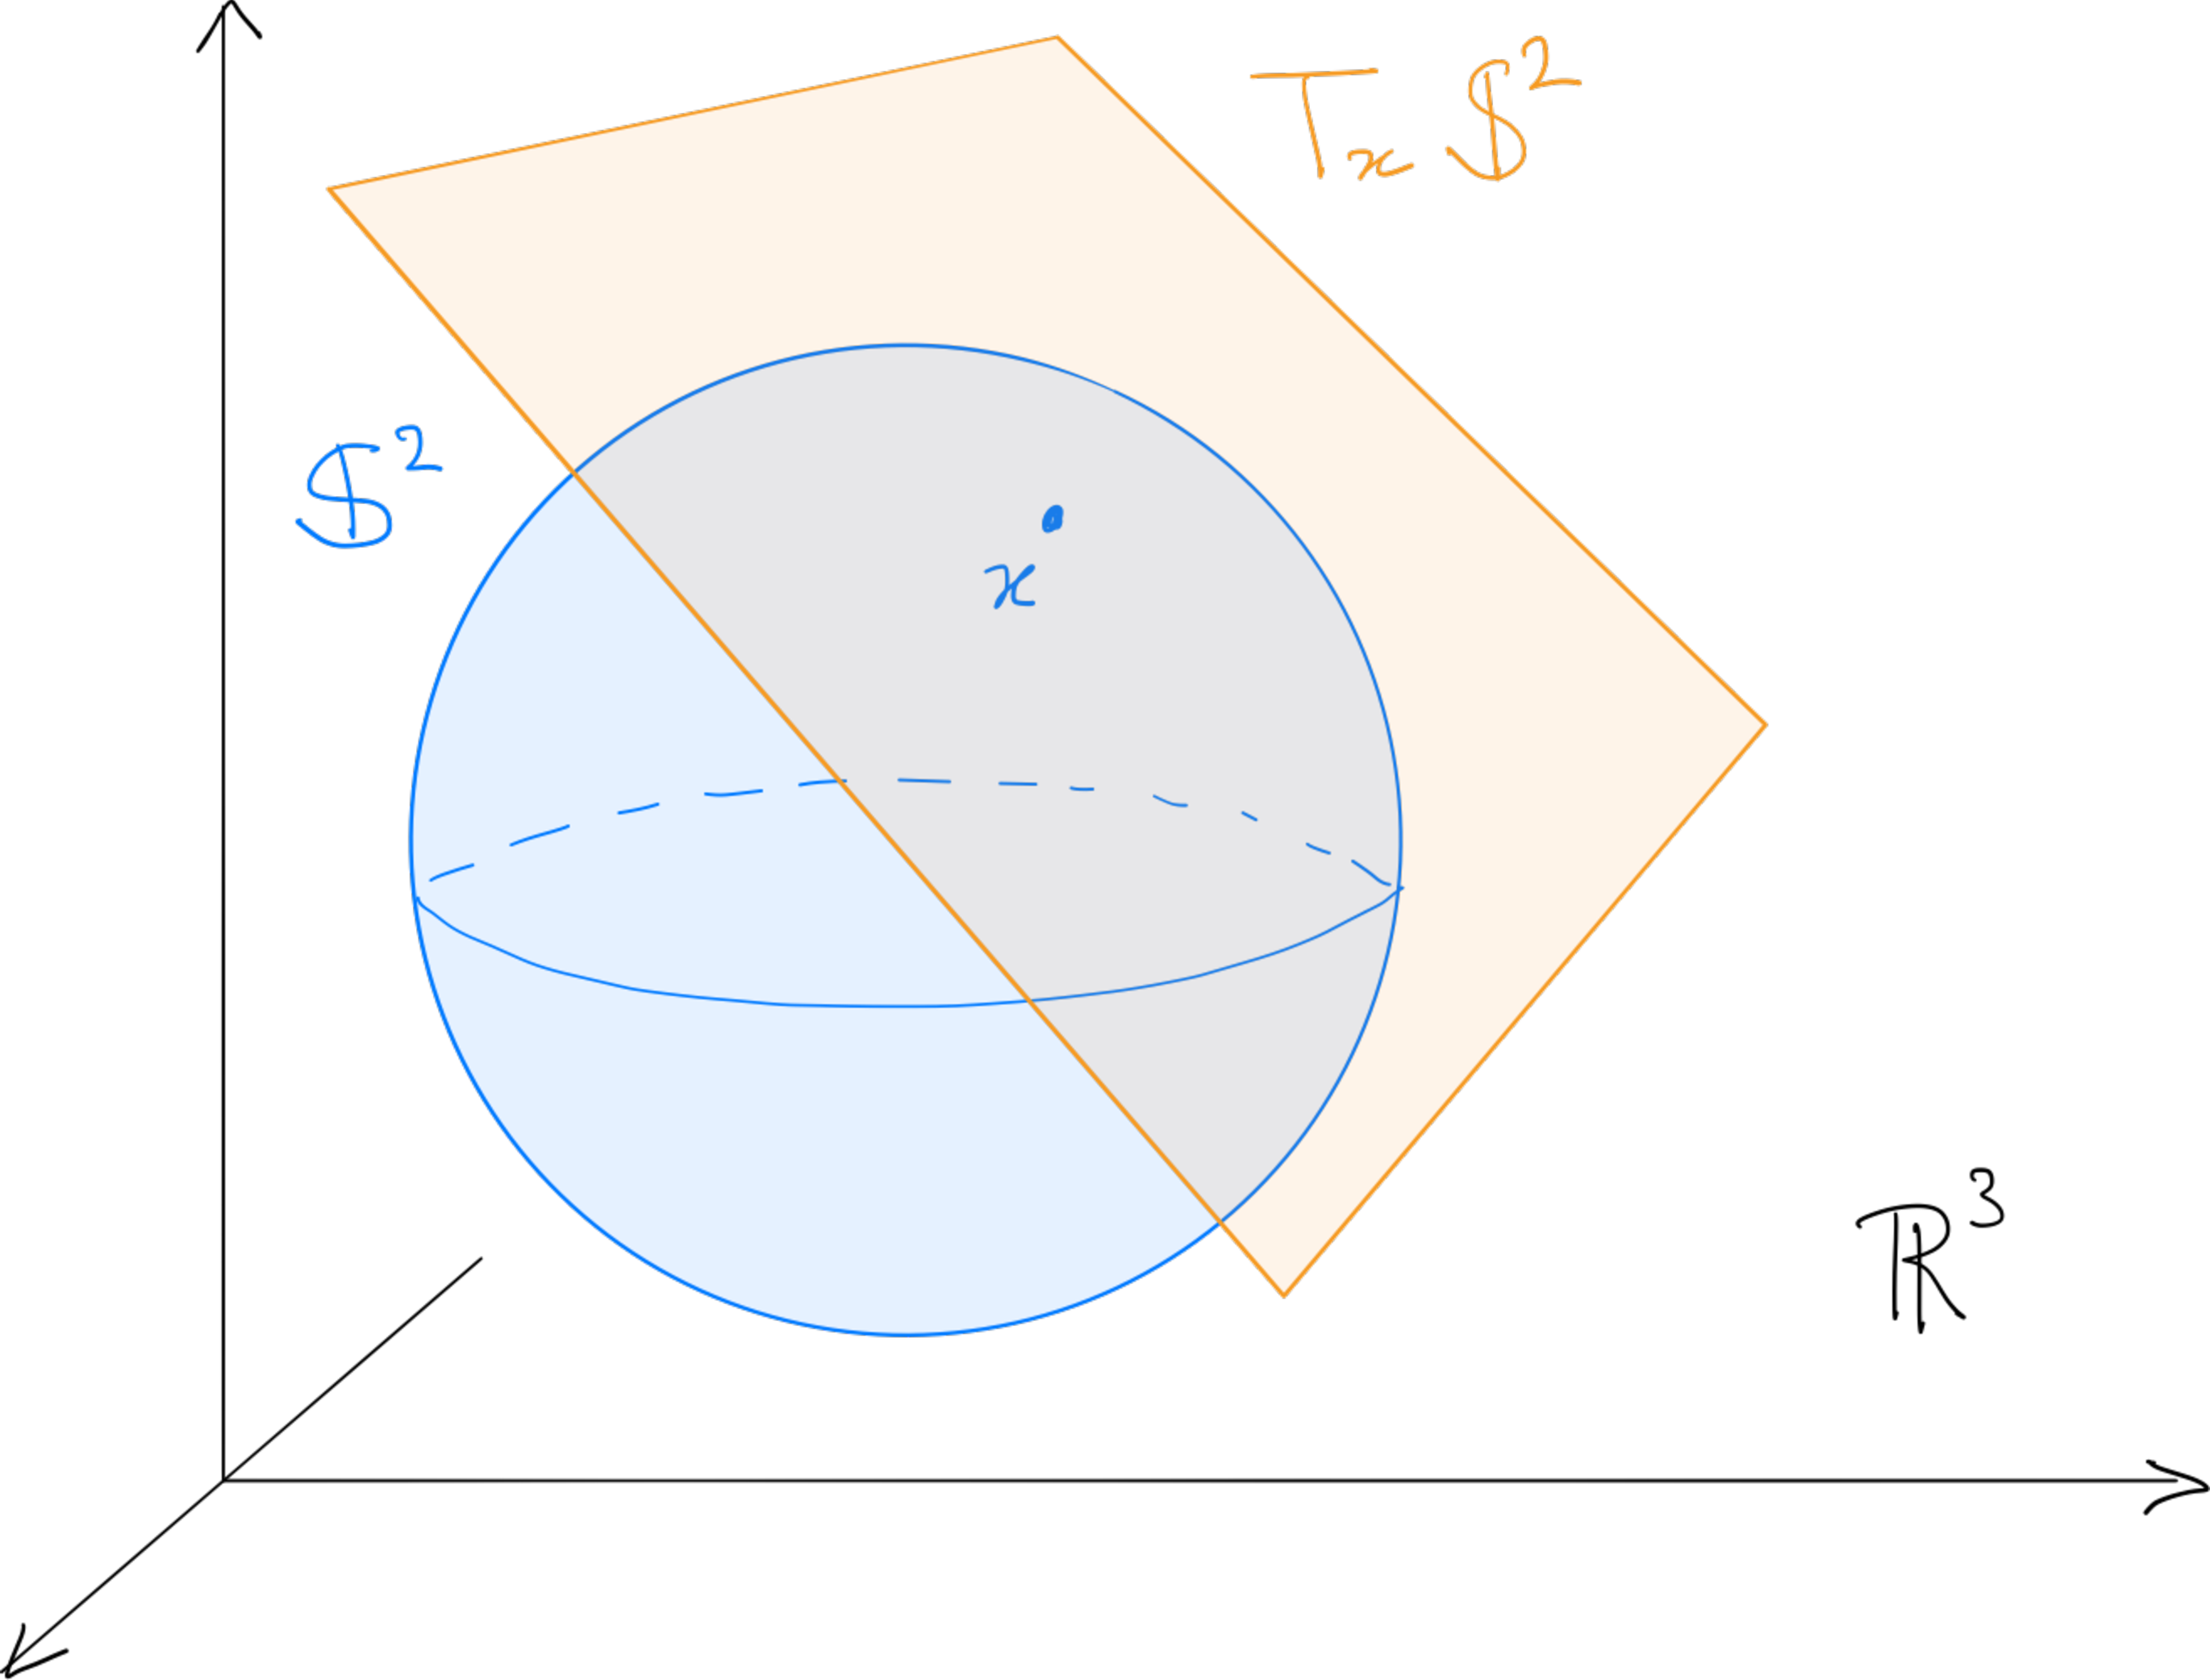
\includegraphics{2_1-embedded-sphere-tangent.pdf}
  \label{fig:tan-embedded-sphere}
  \caption{Tangent space to a point of a sphere $\bS^2$ embedded into the ambient space $\R^3$.}
\end{marginfigure}
In this chapter we will see how to associate to an $n$-dimensional smooth manifold $M$ an $n$-dimensional vector space, denoted by $T_x M$, to each point $x\in M$.
Such vector space is called \emph{tangent space to $M$ at $x$} and, for a manifold embedded into a euclidean ambient space, it will coincide with the intuitive understanding of a tangent hyperplane to the point on the manifold, see also Figure~\ref{fig:tan-embedded-sphere}.
As we will see, there are various different definition of tangent space but, in the end, they all turn out to be equivalent.

Due to the amount of freedom and the many equivalent definitions, there is no unique way of introducing tangent spaces.
Just to give you an idea, all the following approaches lead to equivalent definitions (see also \cite{book:lee}):
\begin{enumerate}
  \item equivalence classes of curves through a point;
  \item transformation laws of the components of vectors with respect to different charts;
  \item generalization of linear approximation into the idea of an abstract derivation;
  \item derivations in the category of germs of functions;
\end{enumerate}

It is also possible to ``flip'' the whole construction around, constructing differentials and cotangent spaces and using them to introduce the tangent spaces.
This is the approach taken by \cite{lectures:hitchin} and it is at least worth of a look if you want to see a different perspective.

To avoid diverging from the book too much, we will stick to derivations on the space of germs, which emphasizes the locality of derivations to an extreme.
The equivalence between our approach and the one based on speeds of curves and on derivations will be left as homeworks.

\section{Directional derivatives in euclidean spaces}\label{sec:dd}

Suppose that $f: U\subset\R^n\to\R^k$ is a smooth map defined on an open subset $U\subset \R^n$.
In multivariable calculus you have seen that if $x\in U$ and $v\in\R^n$, then the vector $Df(x) v$ can be interpreted as the directional derivative\footnote{Sometimes this is denoted $D_v f(x)$ instead.} of $f$:
\begin{equation}
    Df(x) v = \lim_{t\to0}\frac{f(x+tv) - f(x)}{t}.
\end{equation}
Then, the partial derivative is obtained as the particular case
\begin{equation}
    D_jf(x) := Df(x) e_j = \lim_{t\to0} \frac{f(x+te_j) - f(x)}{t}.
\end{equation}
Of course, we can also look at the derivative by using the standard euclidean coordinates $r^1, \ldots, r^n$, in that case we would be deriving $r^i \circ f : \R^n \to \R$.

\newthought{Let's take it slow}, and compare all these various derivatives next to each other.
For $f:U\subset\R^n\to\R^k$ and $x\in U$, we have
\begin{marginfigure}[3.5cm]
    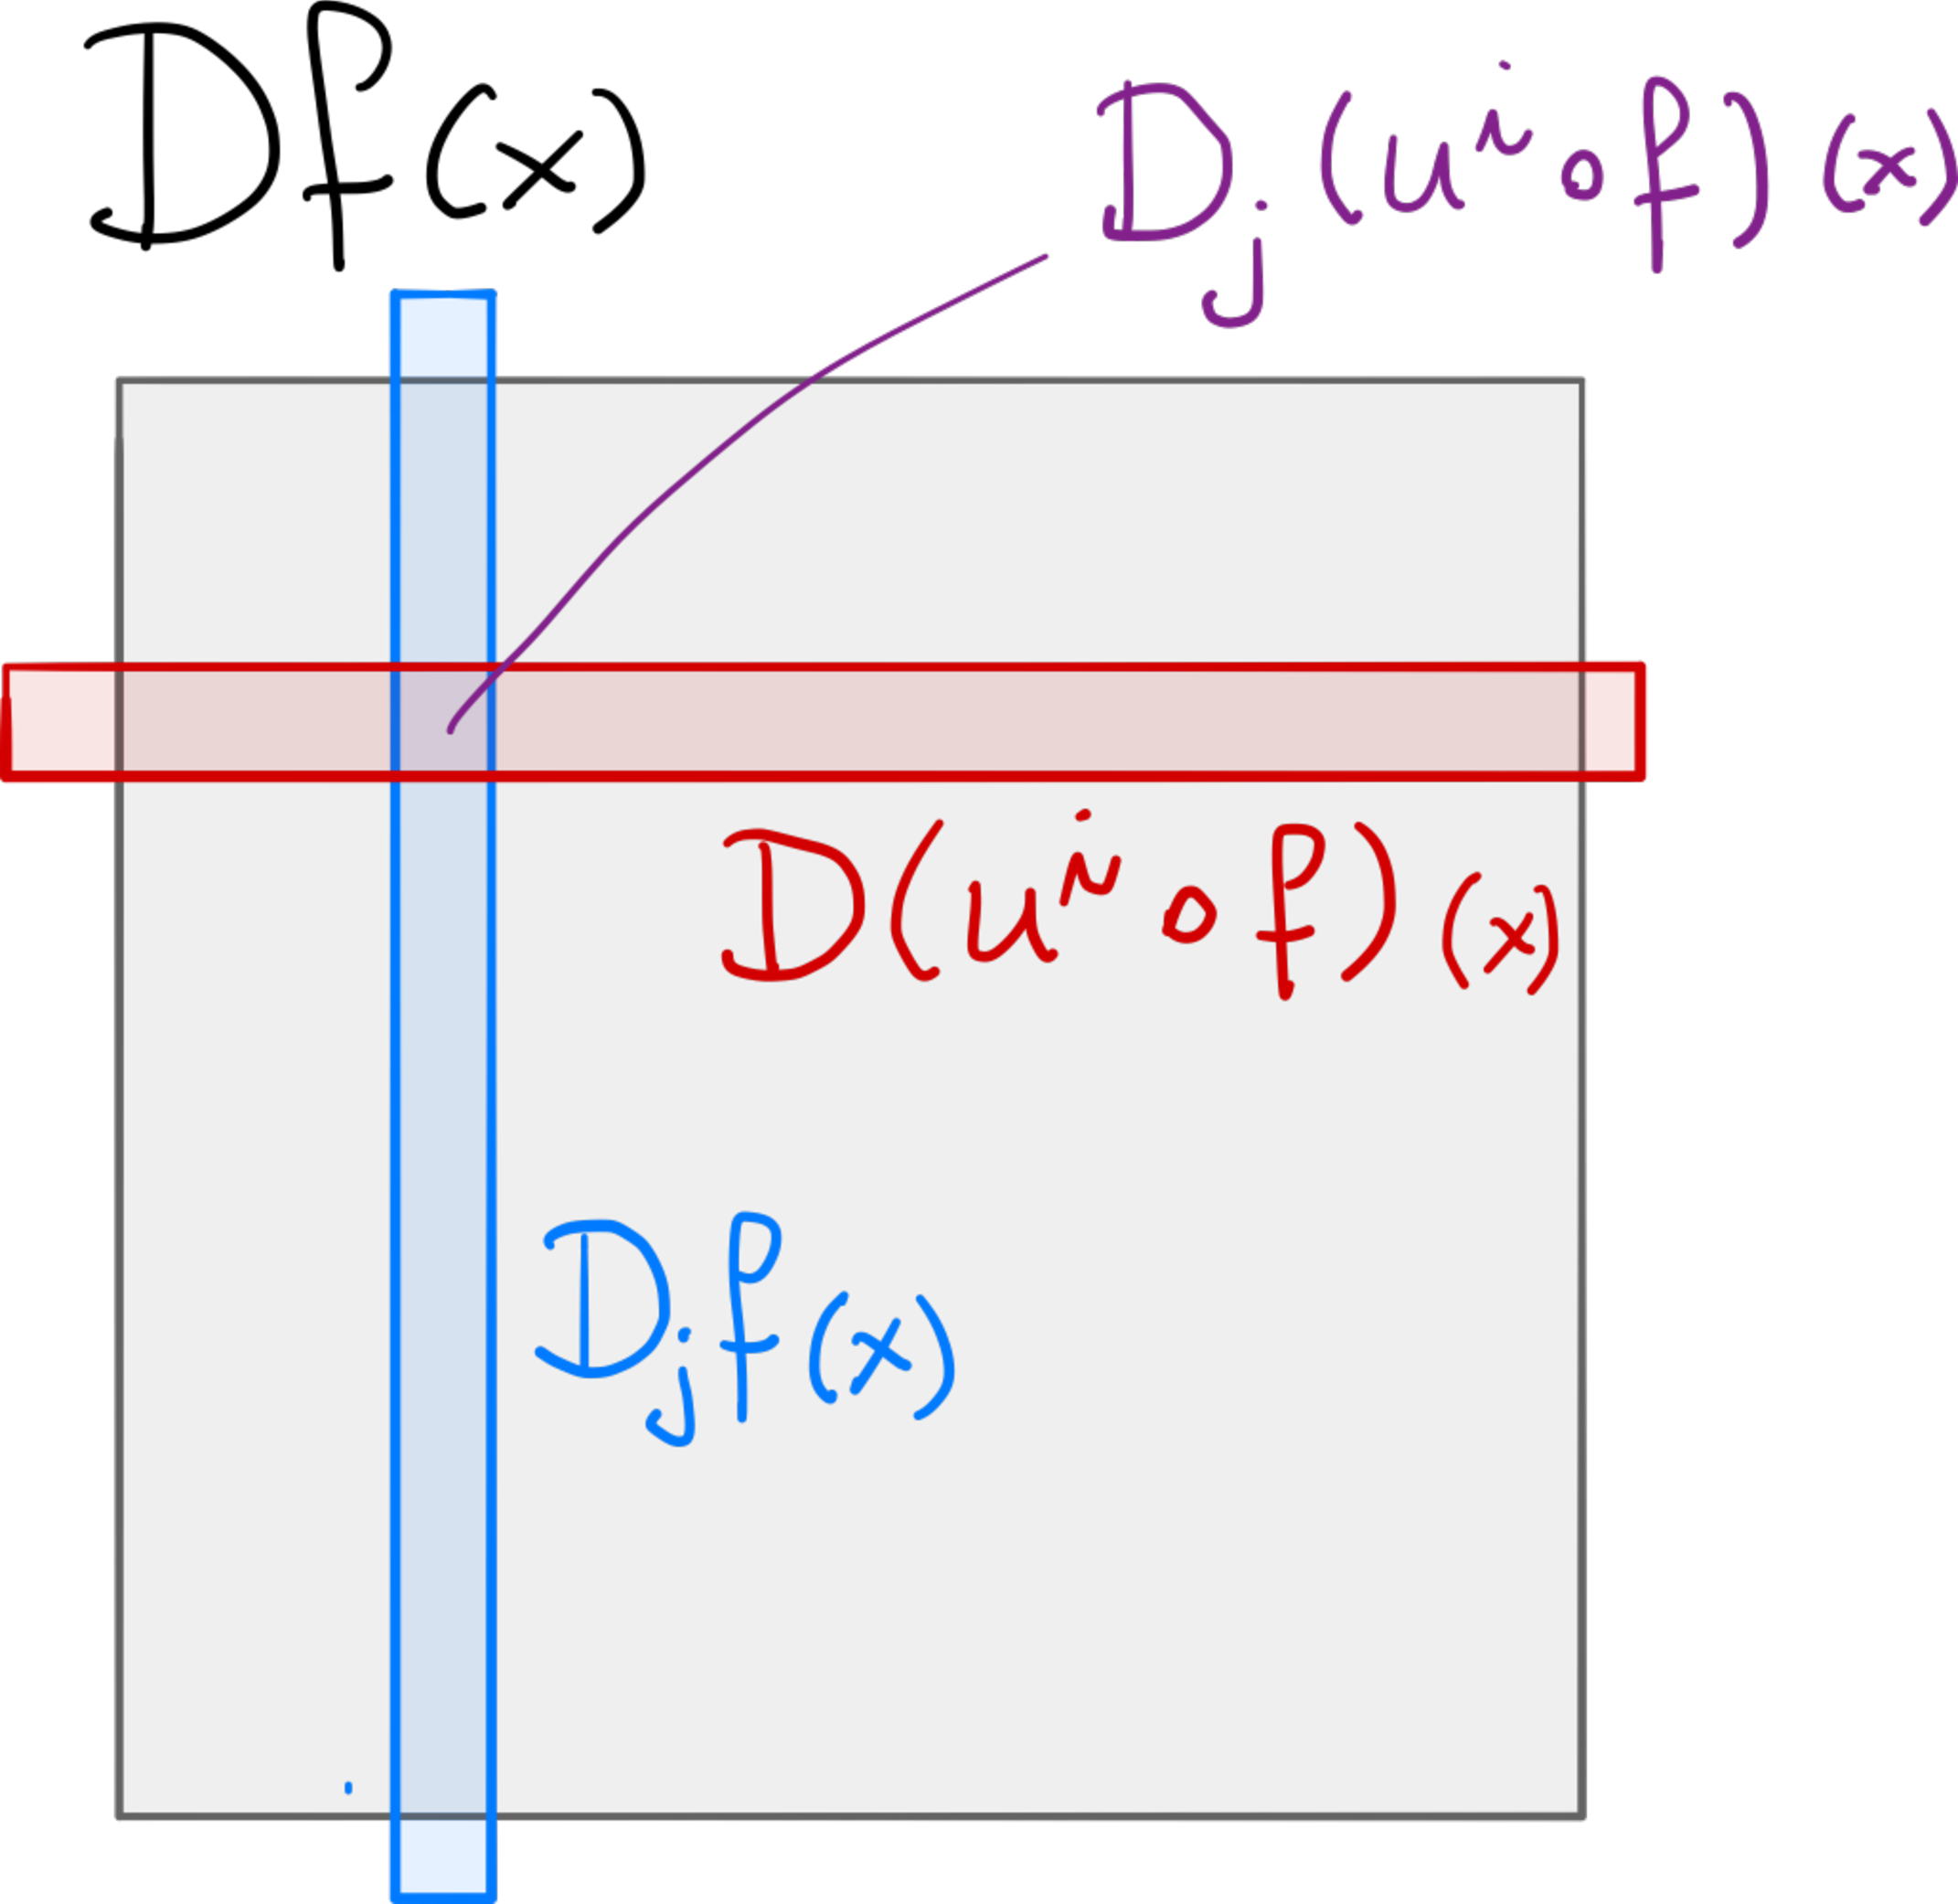
\includegraphics{2_3-ederivs.pdf}
\end{marginfigure}
\begin{itemize}
    \item $Df(x)$, the Jacobian matrix, which is a $k\times n$ matrix;
    \item $D_j f(x)$, the $j$th column of the matrix $Df(x)$, which is an element of $\R^k$;
    \item $D(r^i\circ f)(x)$, a linear function from $\R^n to \R$, which one can think as the $i$th row of the matrix $Df(x)$;
    \item $D_j(r^i\circ f)(x) = \frac{\partial f^i}{\partial x^j}(x)$, a number in $\R$, which corresponds to the element $(i,j)$ of the matrix $Df(x)$.
\end{itemize}

This notation using $D$ instead of spelling out the partial derivatives, comes with an important advantage.
Let's use it to rewrite the chain rule form Proposition~\ref{thm:chainrule}(\ref{thm:chainrule2}):
\begin{equation}
    D_j(u^i\circ g \circ f) (x) = \sum_{r=1}^k D_r(u^i\circ g)(f(x))\; D_j(u^r \circ f)(x),
\end{equation}
\marginnote[-4em]{Using Einstein notation, since $r$ is the only index that appears both in lower and upper position, $D_j(u^i\circ g \circ f) (x) = D_r(u^i\circ g)(f(x))\; D_j(u^r \circ f)(x)$.}
where $1\leq i\leq m, 1\leq j \leq n$.
As you cen see, we did not need to spell out explicitly the coordinate systems on $\R^n$ or $\R^k$.

\section{Germs and derivations}

\newthought{To reach our goal of defining derivations on manifolds}, a direct extension of partial derivatives is not enough: we will need to introduce some more levels of abstraction.

\begin{defn}
    Let $M$ be a smooth manifold.
    For some point $p\in M$, let $U,V\subset M$ be two neighborhoods of $p$.
    We say that two functions $f\in C^\infty(U)$ and $g\in C^\infty(V)$ have the same \emph{germ} at $p$ if there exists a neighborhood $W\subset U\cap V$ of $p$ such that $f|_W \equiv g|_W$.
\end{defn}

Germs define an equivalence relation on the set of smooth functions defined on a neighborhood of a point $p$: $(U, f) \sim_p (V, g)$ if they have the same germ at $p$. Then, a germ $[f]_p$, where $(U, f)$ is one representative for $[f]_p$, is an equivalence class in the quotient space 
\begin{equation}
    C_p^\infty(M) := C^\infty(M)/\sim_p.
\end{equation} 

\begin{exe}
    Show that $\sim_p$ defined above is an equivalence relation in $C^\infty(M)$.
\end{exe}

For $c\in\R$ and $[f]_p, [g]_p$ germs with representatives $(U, f), (V, g)$, we have
\begin{itemize}
    \item $[f]_p + [g]_p$ is the germ with representative $(U\cap V, f+g)$;
    \item $[f]_p [g]_p$ is the germ with representative $(U\cap V, f g)$;
    \item $c[f]_p$ is the germ with representative $(U, cf)$.
\end{itemize}
Therefore, $C_p^\infty(M)$ is also an algebra over $\R$.

Germs are the apotheosis of locality: a germ at $p$ has a well defined value at $p$ and nowhere else.
This results in a map,
\begin{equation}
    \eval_p: C_p^\infty(M) \to \R, \quad
    \eval_p([f]_p) := f(p),
\end{equation}
where $(V,f)$ is any representative of $[f]_p$.

We can now go back to our discussion of euclidean derivations to motivate our definition of tangent vectors.

\begin{ex}\label{ex:euclideanD}
    Let $U\subset\R^n$ open\footnote{In what follows, we will think at $U$ both as an open subset of $\R^n$ and a smooth manifold depending on what is most convenient for us.} and $f\in C^\infty(U)$.
    For $x\in U$ and $v\in\R^n$ we have seen that $Df(x)$ can be interpreted as a matrix that consumes the vector $v$ to produce a number $D(f)v$.
    In such interpretation $f$ is fixed and only $x$ and $v$ vary, however there is no reason for this restriction.

    Indeed, an alternative interpretation lets also $f$ vary and consider the action of differentiation as a map
    \begin{equation}
        U \times \R^n \times C^\infty(U) \to \R,\quad
        (x,v,f) \mapsto Df(x) v.
    \end{equation}
    And since we are flipping around all the ideas, let us consider $x$ and $v$ fixed and instead only let $f$ vary:
    \begin{equation}\label{eq:mapxvtoD}
        (x,v):C^\infty(U) \to\R, \quad (x,v)(f) := Df(x)v.
    \end{equation}.
    By the definition \eqref{eq:diff} of the euclidean differential, we know that it is a local property: the value $Df(x)$ only depends on the germ of $f$ at $x$.
    Thus we can rephrase \eqref{eq:mapxvtoD} by saying that $v$ defines a \emph{linear} map
    \begin{equation}
        v : C_p^\infty(U) \to \R, \quad
        v([f]_p) := Df(x) v.
    \end{equation}
    In fact, this is not just a linear map, it also satisfies a \emph{derivation} property, in the sense that
    \begin{equation}
        v([f]_p [g]_p) =
            \eval_p([f]_p)v([g]_p)
            + \eval_p([g]_p)v([f]_p).
    \end{equation}
    Which, rewritten in a more familiar form, is just a way to rewrite the \emph{Leibniz rule}:
    \begin{equation}
        D(fg)(x) v = f(x)Dg(x)v + g(x) Df(x)v.
    \end{equation}

    Note that we have now two different interpretations for $v$: it is both a vector in $\R^n$ and a linear map $C_p^\infty(U) \to \R$ satisfying the derivation property.
\end{ex}

Motivated by Example~\ref{ex:euclideanD}, we will define a tangent vector as a derivation on the space of germs.

\begin{defn}
    Let $M$ a smooth manifold of dimension $n$ and let $p\in M$.
    A \emph{tangent vector at $p$} is a linear map
    \begin{equation}\label{def:tangentvector}
        v: C_p^\infty(M)\to\R
    \end{equation}
    which is also a derivation, i.e.
    \begin{equation}
        v([f]_p [g]_p) =
            \eval_p([f]_p)v([g]_p)
            + \eval_p([g]_p)v([f]_p).
    \end{equation}

    Since a tangent vector is a linear map from the vector space $C_p^\infty(M)$ to $\R$, the set of all tangent vectors at a point $p$ is itself a vector space\footnote{Exercise: why is this true?} which we denote by $T_p M$.
\end{defn}

Let's check that these vectors, at least satisfy the most elementary properties of derivations: one would expect the derivative of constant functions to be zero, is that the case?

\begin{lem}\label{lem:f'0is0forconst}
    Let $M$ be a smooth manifold, let $U\subset M$ be an open set containing $p$ and let $v\in T_p M$.
    Denote by $[c]_p$ the germ of a constant function $(U, p \mapsto c)$.
    Then $v([c]_p) = 0$.
\end{lem}
\begin{proof}
    Since $[c]_p = c [1]_p$, by linearity we have $v([c]_p) = c v([1]_p)$.
    Thus, it will be enough to show that $v([1]_p) = 0$.
    Since $v$ is a derivation, using the algebra properties of the space of germs we get
    \marginnote{Keep this simple trick in mind, it will be useful in the future.}
    \begin{equation}
        v([1]_p) = v([1]_p [1]_p) = 2 \eval_p([1]_p)v([1]_p) = 2 v([1]_p).
    \end{equation}
    Thus, $v([1]_p) = 0$, concluding the proof.
\end{proof}

As you can see, working with equivalent classes is doable but unnecessarily cumbersome. As we did with atlases, we would like to get it over with.

\begin{defn}
    Let $M$ be a smooth manifold and $p\in M$.
    Let $W\subseteq M$ be any neighborhoods of $p$.
    A \emph{derivation of $C^\infty(W)$ at $x$} is a linear map $w:C^\infty(W)\to\R$ which satisfies Leibniz rule
    \begin{equation}
        w(fg) = f(p)w(g) + g(p)w(f).
    \end{equation}
\end{defn}

If $v\in T_p M$, then we already saw that $v$ naturally defines a derivation $w$ of $C^\infty(W)$ for any open neighborhood $W$ of $p$.
In this case
\begin{equation}\label{eq:derivfromtg}
    w(f) := v([f]_p).
\end{equation}
Showing that the opposite is also true will require a bit of work.

\begin{prop}
    Let $M$ be a smooth manifold, $p\in M$ and $W$ any neighborhood of $x$.
    Then there is a linear isomorphism between $T_p M$ and the space of derivations of $C^\infty(W)$ at $p$.
\end{prop}
\begin{proof}
    To prove the theorem we need to invert \eqref{eq:derivfromtg} and define a tangent vector in terms of of a derivation of $C^infty(W)$ at $p$.
    We will proceed in three steps

    \newthought{Step I}. Let $w:C^\infty(W) \to\R$ be a derivation at $p$ and suppose that $f\in C^\infty(W)$ is identically zero on a neighborhood $W_0\subset W$ op $p$. We are going to show that $w(f)=0$.

    By Proposition~\ref{prop:cutoff}, we can find a function $\rho:M\to\R$ such that $\rho(p)=1$ and $\supp(\rho) \subset W_0$. Consider now $g = \rho f : W \to \R$. Then $g$ is identically zero in the whole $W$, and thus\footnote{Follows by linearity, exactly as in Lemma~\ref{lem:f'0is0forconst}} $w(g) = 0$. Using Leibniz rule, the fact that $\rho(p)=1$ and $f(p) = 0$, we get
    \begin{equation}
        0 = w(g) = w(\rho f) = \rho(p) w(f) + f(p)w(\rho) = w(f).
    \end{equation}

    \newthought{Step II}.
    Let $[f]_p\in C_p^\infty(M)$.
    We want to show that it is always possible to find a representative for $[f]_p$ with domain $W$, that is, there exists $g\in C^\infty(W)\to\R$ such that $[g]_p = [f]_p$.
    Let $(V, f)$ be any representative of $[f]_p$.
    Since germs are local, if necessary, we can shrink $V$ so that $V\subset W$.
    Here comes the tricky bit: we need to extend $f$ to a function $g$ defined on $W$ which coincides with $f$ in some neighborhood of $p$!
    To this end, choose\footnote{We can do this because topological manifolds are locally compact Hausdorff spaces, which implies that every point has a neighborhood with compact closure.} a smaller neighborhood $U$ of $p$ such that $\overline{U}\subset V\subset W$.
    Again, Proposition~\ref{prop:cutoff} comes to the rescue. Apply it with $K=\overline{U}$ and ``$U$'' equal to $V$, and consider
    \begin{equation}
        g:W\to\R, \quad
        g(q) := \begin{cases}
            \rho(q)f(q), & q\in V,\\
            0, & q \in W\setminus V.
        \end{cases}
    \end{equation}
    Since $g|_U = f$, we have $[g]_p = [f]_p$, proving the claim.

    \newthought{Step III}. We can now complete the proof.
    Let $w:X^\infty(W) \to\R$ be a derivation at $p$.
    A tangent vector is a linear map $v:C_p^\infty(M)\to\R$, see \eqref{def:tangentvector}, and a derivation.
    We would like to define one in terms of $w$.
    Given any $[f]_p\in C_p^\infty(W)$, the previous step guarantees that there exists a representative $(W,f)$ for it, so we can define
    \begin{equation}
        v([f]_p) := w(f), \quad\mbox{where $(W,f)$ is any representative of $[f]_p$}.
    \end{equation}
    Such $v$ is a derivation by construction, so if it is well-defined, we are done.
    To this end, assume that there exists a different representative $(W, g)$ for $[f]_p$.
    Then, by definition, there exists a neighborhood $V\subset W$ of $p$ such that $f|_p = g|_p$.
    By linearity, $w(f) - w(g) = w(f-g)$ and by the first step in the proof, $w(f-g) = 0$.
    
    The assignment $w\mapsto v$ inverts \eqref{eq:derivfromtg}, completing the proof.
\end{proof}

This seemingly innocent proposition, has some very important consequences.

First of all, from now on we are free to interpret tangent vectors in $T_p M$ as derivations of $C^\infty(W)$ at $p$ for \emph{any}\footnote{In particular, it is often convenient to have $W$ coincide with the domain of a chart or with the whole manifold $M$.} open $W$ containing $p$.
This enables us to give our first example of tangent vector.

\begin{ex}\label{ex:partialderivative}
    Let $M$ be a smooth manifold of dimension $n$ and $\phi: U \to V$ a chart on $M$.
    As already mentioned, we write $x^i = r^i \circ \phi$ for the local coordinates\footnote{See Notation~\ref{ntn:coords}.} of $\phi$.
    For any $p\in U$, we can define a derivation of $C^\infty(U)$ at $p$ as
    \begin{equation}
        \frac{\partial}{\partial x^i}\Big|_p : C^\infty(U) \to \R, \quad
        \frac{\partial}{\partial x^i}\Big|_p (f) := D_i(f\circ\phi^{-1})(\phi(p)).
    \end{equation}
    We will soon see that $\left\{\frac{\partial}{\partial x^i}\Big|_p \mid 1\leq i\leq n\right\}$ forms a basis for $T_p M$.
\end{ex}

Secondly, it provides us some very useful corollaries.

\begin{cor}\label{cor:tgsubspace}
    Let $M$ be a smooth manifold and let $W\subset M$ be a non-empty open set considered as a smooth manifold.
    Then, for any $p\in W$ there is a canonical identification $T_pW = T_p M$.
\end{cor}

\begin{cor}\label{cor:derzero}
    Let $M$ be a smooth manifold and $p\in M$.
    Let $W\subseteq M$ be an open neighborhoods of $p$.
    If $f\in C^\infty(W)$ is constant in a neighborhood of $p$, then $v(f) = 0$ for all $v\in T_p M$.
\end{cor}

With these new tools at hand, we are ready to state and prove an important result on the size of the tangent spaces.
As it turns out, $T_pM$ is a finite dimensional vector space, naturally isomorphic to $\R^n$.

\begin{thm}\label{thm:dimensionTpM}
    Let $M$ be a smooth manifold of dimension $n$ and $p\in M$.
    Then $T_pM$ is a vector space of dimension $n$.
\end{thm}

The theorem will follow immediately once we construct a basis for $T_pM$.
To that end, we need a preliminary result from multivariable analysis.

\begin{lem}\label{lem:Taylor}
    Let $U\subset\R^n$, $0\in U$, be a star-shaped\footnote{An open set $U\subset\R^n$ containing the origin, $0\in U$, is called \emph{star-shaped} if $U$ also contains the line segment from $0$ to $x$ for any $x\in U$.} open set.
    Then, there exists $n$ smooth functions $g_i: U \to \R$, $1\leq i \leq n$, such that $g_i(0) = D_i h(0)$ and
    \begin{equation}
        h = h(0) + r^i g_i
    \end{equation}
    \marginnote[-1.8em]{$\leftarrow$ This is our first use of Einstein notation, this equation should be read as $h(x) = h(0) + \sum_{i=1}^n r^i(x) g_i(x)$.
    Using the global euclidean chart, $x^i = r^i(x)$ and $h(x) = h(0) + \sum_{i=1}^n x^i g_i(x)$, which you may recognize as the first iteration of the usual Taylor-MacLaurin formula.}
    where $r^i$ are the coordinates introduced in Notation~\ref{ntn:coords}.
\end{lem}
\begin{proof}
    Fix a point $x = (x^1, \ldots, x^n) \in U$.
    Let $\gamma_x:[0,1]\to U$ denote the line segment from $0$ to $x$, parametrized as $\gamma_x(t) = tx$.

    By the chain rule,
    \begin{equation}
        \frac{d}{dt}(h \circ \gamma_x) (t) = \left(D_i h(t x)\right) \times \frac{d}{dt} (t x^i)' = x^i D_i h(t x).
    \end{equation}
    \marginnote[-2.5em]{$\leftarrow$ Again, due to Einstein notation, the right hand side should be read as $\sum_{i=1}^n x^i D_i h(t x)$.}
    The fundamental theorem of calculus then implies
    \begin{align}
        h(x) - h(0) &= (h \circ \gamma_x)(1) - (h \circ \gamma_x)(0) \\
        &= \int_0^1 (h \circ \gamma_x)(t)\;dt = x^i \int_0^1 D_i h(tx)\; dt.
    \end{align}
    \marginnote[-2.1em]{$\leftarrow$ For one last time, due to Einstein notation, the right hand side should be read as $\sum_{i=1}^n x^i \int_0^1 D_i h(t x)\; dt$.}

    Since $x^i = r^i(x)$ by definition, the theorem follows by defining
    \begin{equation}
        g_i(x) := \int_0^1 D_i h(tx)\; dt.
    \end{equation}
\end{proof}

Theorem~\ref{thm:dimensionTpM} now follows from the next statement.

\begin{prop}\label{prop:basis_TpM}
    Let $M$ be a smooth manifold of dimension $n$ and $p\in M$.
    Let $\phi: U \to V$ be a chart on $M$ around $p$, i.e. $p\in U$.
    Then any tangent vector $v\in T_p M$ can be uniquely written as a linear combination
    \begin{equation}
        v = v^i \frac{\partial}{\partial x^i}\Big|_p, \quad v_i = v(x^i).
    \end{equation}
    \marginnote[-3em]{$\leftarrow$ Since we consider upper indices in the denominator as lower indices, the equation should be read as $v = \sum_{i=1}^n v^i \frac{\partial}{\partial x^i}\Big|_p$. If $M=\R^n$, what we are saying here is that $v(f) = v\cdot\nabla f = Df\; v$, that is, $v$ acts as the directional derivative in its direction.}
    Thus, $\left\{\frac{\partial}{\partial x^i}\Big|_p\;\mid\; 1\leq i\leq n\right\}$ is a basis of $T_p M$.
\end{prop}
\begin{proof}
    We may assume without loss of generality that $\phi(p) = 0$ and, thanks to Corollary~\ref{cor:tgsubspace}, $U$ is star-shaped.
    Let $f\in C^\infty(U)$.
    By Lemma~\ref{lem:Taylor} with $h = f \circ \phi^{-1}$ we get
    \begin{equation}
        f = f(p) + x^i (g_i \circ \phi),
        \quad g_i(0) = D_i (f \circ \phi^{-1})(0) = \frac{\partial}{\partial x_i}\Big|_p(f).
    \end{equation}
    Thus, for any derivation $v$, we obtain
    \begin{equation}
        v(f) = v(f(p)) + v(x^i)g_i(0) + x^i(p) v(g_i\circ\phi) = v(x^i)  \frac{\partial}{\partial x_i}\Big|_p(f).
    \end{equation}
    The right hand side is obtained observing that $\phi(p) = 0$, and thus the components $x^i(p) = 0$ are all zero, and applying Corollary~\ref{cor:derzero} to the constant $f(p)$, which implies $v(f(p)) = 0$.
    
    It follows that the set $\left\{\frac{\partial}{\partial x^i}\Big|_p\;\mid\; 1\leq i\leq n\right\}$ spans $T_p M$.
    We now need to show that its elements are linearly independent.
    Observe that
    \begin{align}
        \frac{\partial}{\partial x_i}\Big|_p (x^j) &= 
        \frac{\partial}{\partial x_i}\Big|_p (r^j \circ \phi)\\
        &= D_i (r^j \circ \phi \circ \phi^{-1}) (\phi(p))\\
        &= D_i r^j(\phi(p)) = \delta^j_i.
    \end{align}
    Thus, if
    \begin{equation}
        v = a_i \frac{\partial}{\partial x_i}\Big|_p,
    \end{equation}
    by letting $v$ act on $x^j$, $j\leq 1\leq n$, we obtain $(a_1, \ldots, a_n) = 0$, proving the linear independence.
\end{proof}

\begin{rmk}[Change of coordinates]
    Suppose $\phi$ and $\psi$ are two different charts about $p$, with corresponding coordinates $x^i := r^i \circ \phi$ and $y^i := r^i \circ \psi$.
    Taking $v = \frac{\partial}{\partial y^j}\Big|_p$ in the previous proposition implies that
    \begin{equation}
        \frac{\partial}{\partial y^j}\Big|_p = 
        \frac{\partial}{\partial y^j}\Big|_p (x^i) \frac{\partial}{\partial x^i}\Big|_p.
    \end{equation}
    \marginnote[-3em]{If we start getting used to these vectors as actual derivatives and hide the dependence on $p$, then this equation can be rewritten as $\frac{\partial}{\partial y^j} = 
    \frac{\partial x^i}{\partial y^j} \frac{\partial}{\partial x^i}$.}

    If we expand the definitions, we get
    \begin{equation}
        \frac{\partial}{\partial y^j}\Big|_p (x^i) =
        D_j(x^i\circ\psi^{-1})(\psi(p)) =
        D_j(r^i \circ \phi \circ \psi^{-1})(\psi(p)),
    \end{equation}
    which is the $(i,j)$th entry in the matrix $D(\phi\circ\psi^{-1})(\psi(p))$ as discussed at the beginning of Section~\ref{sec:dd}.

    In other words, $D(\phi\circ\psi^{-1})(\psi(p))$ is the transition matrix from the basis $\left\{\frac{\partial}{\partial y^i}\Big|_p\;\mid\; 1\leq i\leq n\right\}$ to the basis $\left\{\frac{\partial}{\partial x^i}\Big|_p\;\mid\; 1\leq i\leq n\right\}$.
\end{rmk}

We said in the introduction that there are multiple equivalent definition of the tangent space. In the following exercise you will provide one in terms of charts and euclidean derivatives.
Soon, we will see yet another definition.

\begin{exe}\label{exe:vsstruct}
    Let $\{V_\alpha \mid \alpha\in A\}$ be a family of vector spaces indexed by a set $A$, let $W$ be a fixed set and let $T_\alpha: V_\alpha\to W$ be a bijection for all $\alpha\in A$.
    Assume that for any $\alpha, \beta \in A$, the composition $T_\beta^{-1}\circ T_\alpha : V_\alpha \to V_\beta$ is a linear isomorphism.
    Show that there is a unique vector space structure on $W$ such that each $T_\alpha$ is a linear isomorphism.
\end{exe}

\begin{exe}[Tangent vectors as equivalence classes of charts and vectors]
Let $M$ be a smooth $m$-manifolds with maximal smooth atlas $\Sigma$.
For $p\in M$, let $\Sigma_p \subset \Sigma$ denote the set of charts $\phi\in\Sigma$ such that $p$ lies in the image of $\phi$.
\begin{enumerate}
    \item Show that
    \begin{equation}
        (v,\phi) \sim (w, \psi)
        \quad\Longleftrightarrow\quad
        D(\psi \circ \phi^{-1})(\phi(p))v = w.
    \end{equation}
    defines an equivalence relation on $\R^m\times\Sigma_p$.
    \item Let $\cT_p$ denote the set of equivalence classes $[(v,\phi)]\in \R^m\times\Sigma_p/\sim$. For $\phi\in\Sigma_p$, show that the map $T_\phi:\R^m\to\cT_p$ given by $T_\phi v := [(v,\phi)]$ is a bijection.
    Deduce\footnote{Hint: use the previous exercise!} that $\cT_p$ admits a unique vector space structure such that each $T_\phi$ is a linear isomorphism.
    \item Let $\phi$ be a chart defined on a neighborhood of $p$ with local coordinates $x^i = r^i \circ \phi$ and let $\hat T_\phi :\R^m \to T_pM$ denote\footnote{As it turns out, this is the same as $T_x$ defined in \eqref{def:lin_iso_Tp}, however in this exercise we use a different notation to emphasize the dependence on the chart.} the linear isomorphism defined by $\hat T_\phi e_i = \frac{\partial}{\partial x^i}\big|_p$.
    Show that there exists a linear isomorphism $\mathcal{S}_p:\cT_p\to T_pM$ which in addition satisfies $\mathcal{S}_p \circ T_\phi = \hat T_\phi$ for every chart $\phi$ about $p$.
\end{enumerate}
\end{exe}

\section{The differential of a smooth map}

\newthought{In the case of a smooth map between Euclidean spaces}, the total derivative of the map at a point (represented by its Jacobian matrix) is a linear map that represents the best linear approximation to the map near the given point.
In the manifold case there is a similar linear map but, as we discussed, it makes no sense to talk about a linear map between manifolds: we need to find a suitable linear map between tangent spaces.

It should not come a surprise that with the constructions developed so-far not only we have one such map, but we can directly relate it to a derivative.

\begin{defn}
    Let $F: M \to N$ be a smooth map between the smooth manifolds $M$ and $N$.
    Let $p\in M$. The \emph{differential $d F_p$ of $F$ at $p$} is the map\footnote{In the differential geometry literature, the differential has many names: you can find it called \emph{tangent map}, \emph{total derivative} or \emph{derivative} of $F$. Since it ``pushes'' tangent vectors forward from the domain manifold to the codomain, it is also called the \emph{pushforward}. If that was not enough, different authors use different notation for it: besides $dF_p(v)$, you can find $F_* v_p$, $F'(p)$, $T_pF$, $DF(p)[v]$ or variations thereof.}
    \begin{equation}
        d F_p : T_p M \to T_{F(p)} N, \qquad d F_p (v) (f) := v(f\circ F), \quad \forall f\in C^\infty(N).
    \end{equation}    
\end{defn}

Indeed, $v \mapsto d F_p (v)$ is a linear map (why?) defining a derivation at $F(p)$ acting on functions in $C^\infty(N)$ (why?) and, as such, is also a tangent vector in $T_F(p)N$.

\begin{exe}
    Answer the two \emph{(why?)} above.
\end{exe}

\begin{thm}[The chain rule on manifolds]
    Let $M, N, P$ be smooth manifolds and $F: M \to N$, $G: N\to P$ be two smooth maps. Then
    \marginnote{The alternative $D$ notation, in this case, makes the relation to the usual chain rule even more evident: $D(G\circ F)(p) = DG(F(p))\circ DF(p)$.}
    \begin{equation}
        d(G\circ F)_p = dG_{F(p)} \circ dF_p.
    \end{equation}
\end{thm}
\begin{proof}
    Since $dF_p : T_p M \to T_{F(p)}N$ and $dG_{F(p)}: T_{F(p)}N \to T_{G(F(p))}P$, the map $d(G\circ F)_p: T_p M \to T_{G(F(p))}P$ has the right domain and codomain.
    Take now $v\in T_p M$ and $f\in C^\infty(L)$. We get
    \begin{align}
        d(G\circ F)_p(v)(f) &= v(f\circ G \circ F)
        = dF_p (v)(f\circ G) \\
        &\stackrel{\star}{=} dG_{F(p)}(dF_p (v))f 
        = dG_{F(p)} \circ dF_p,
    \end{align}
    where in $\star$ we used the fact that $dF_p (v)\in T_{F(p)}N$.
\end{proof}

\begin{rmk}
    The differential of the identity map $\id_M:M\to M$ at any point $p\in M$ is the identity map
    \begin{equation}
        \id_{T_pM}: T_pM \to T_pM.
    \end{equation}
    Indeed, $d (\id_M)_p(v)(f) = v(f\circ\id_M) = v(f)$ for any $v\in T_pM$ and any $f\in C^\infty(M)$.
\end{rmk}

The definition we gave seems quite abstract, let's see what it looks like in coordinates.

\begin{prop}\label{prop:DiffCoords}
    Let $F:M^m\to N^n$ be a smooth map between smooth manifolds.
    Let $p\in M$, and let $\phi : U \to \phi(U)$ be a chart on $M$ about $p$ and $\psi: V \to \psi(V)$ be a chart on $N$ about $F(p)$.
    If $(x^i)$ denote the local coordinates of $\phi$ and $(y^i)$ the ones of $\psi$, the matrix of $dF_p$ with respect to the bases $\left\{\frac{\partial}{\partial x^j}\big|_p \;\mid\; j=1,\ldots,m\right\}$ of $T_pM$ and $\left\{\frac{\partial}{\partial y^j}\big|_p \;\mid\; j=1,\ldots,n\right\}$ of $T_{F(p)}N$ is given by the Jacobian matrix $D(\psi\circ F \circ\phi^{-1})(\phi(p))$.
\end{prop}
\begin{proof}
    The proof follows from the following direct computation after observing that the number $D_j(r^i \circ \psi \circ F \circ \phi^{-1})(\phi(p))$ is the $(i,j)$ entry of the Jacobian matrix $D(\psi\circ F \circ\phi^{-1})(\phi(p))$. For any $j=1,\ldots,m$,
    \begin{align}
        dF_p \left(\frac{\partial}{\partial x^j}\Big|_p\right)
        &= \sum_{i=1}^n dF_p \left(\frac{\partial}{\partial x^j}\Big|_p\right) (y^i) \frac{\partial}{\partial y^i}\Big|_{F(p)} \\
        &= \sum_{i=1}^n \frac{\partial}{\partial x^j}\Big|_p (y^i \circ F) \frac{\partial}{\partial y^i}\Big|_{F(p)} \\
        &=\sum_{i=1}^n D_j(r^i \circ \psi \circ F \circ \phi^{-1})(\phi(p)) \frac{\partial}{\partial y^i}\Big|_{F(p)}.
    \end{align}
\end{proof}

\begin{exe}
    Show that the matrix of $d F_p$ in terms of the coordinate bases is 
    \begin{equation}
        \begin{pmatrix}
            \frac{\partial F^1}{\partial x^1} (p) & \cdot & \frac{\partial F^1}{\partial x^n} (p) \\
            \vdots & \ddots & \vdots \\
            \frac{\partial F^m}{\partial x^1} (p) & \cdot & \frac{\partial F^m}{\partial x^n} (p)
        \end{pmatrix}
    \end{equation}
    without using the Proposition above.

    \noindent Hint: show that $d F_p \left(\frac{\partial}{\partial x^i}\big|_p\right) (f) = \left(\frac{\partial F^j}{\partial x^i} (p) \frac{\partial}{\partial y^j}\big|_{F(p)}\right) (f)$.
\end{exe}

\newthought{A particularly important consequence} of this theorem is that our definition coincides with our old euclidean notions if we set $M=\R^m$ and $N=\R^n$.
This is easily checked by taking $\phi = \id_{\R^m}$ and $\psi=\id_{\R^n}$.
Then the coordinates $(x^1,\ldots,x^m)$ are the standard euclidean coordinates for $\R^m$ and the coordinates $(y^1,\ldots,y^n)$ the ones for $\R^n$.

Let $f:U\subset\R^m\to\R^n$ be a smooth function and define the linear isomorphisms
\begin{align}\label{def:lin_iso_Tp}
    &T_x : \R^m \to T_x\R^m,\quad T_x e_i = \frac{\partial}{\partial x^i}\Big|_x,\\
    &T_y : \R^n \to T_y\R^n,\quad T_y e_i' = \frac{\partial}{\partial y^i}\Big|_y
\end{align}
where $\{e_1,\ldots,e_m\}$ denotes the standard basis of $\R^m$ and $\{e_1',\ldots,e_m'\}$ denotes the standard basis of $\R^n$.

On the one hand, we have the total derivative $Df(x):\R^m\to\R^n$ from multivariable calculus: a linear map, the Jacobian matrix of partial derivatives.
On the other, we have the differential $df_x : T_x \R^m \to T_{f(x)}\R^m$ defined above: also a linear map, related to the Jacobian matrix of partial derivatives by Proposition~\ref{prop:DiffCoords}.
In fact we know more, since Proposition~\ref{prop:DiffCoords} tells us that the following diagram commutes:
\begin{equation}
    \begin{tikzcd}[row sep=huge, column sep=huge]
        \R^m \arrow[r, "Df(x)"] \arrow[d, "T_x"]
        & \R^n \arrow[d, "T_{f(x)}"] \\
        T_x\R^m \arrow[r, "df_x"]
        & T_{f(x)}\R^n
    \end{tikzcd}.
\end{equation}

More generally, the same kind of computation shows the following fact. For any smooth map $F:M^m \to N^n$ between smooth manifolds, if $\phi$ is a chart about $p\in M$ with coordinates $(x^i)$ and $\psi$ is a chart about $F(p)\in N$ with coordinates $(y^i)$, the following diagram commute:
\begin{equation}
    \begin{tikzcd}[row sep=huge, column sep=huge]
        \R^m \arrow[r, "D(\psi \circ F \circ \phi^{-1})(\phi(x))"] \arrow[d, "T_x"]
        & \R^n \arrow[d, "T_{F(x)}"] \\
        T_xM \arrow[r, "dF_x"]
        & T_{f(x)}N
    \end{tikzcd},
\end{equation}
where $T_p$ and $T_{F(p)}$ are defined as above.

The construction that we employed forced us to fix a basis for the spaces, if this was truly necessary it would defeat the purpose of this whole chapter.
Fortunately for us, the following exercise shows that, at any given point, the tangent space to a vector space is \emph{canonically}\footnote{That is, independently of the choice of basis.} identified with the vector space itself.

\begin{exe}
    Let $V$ and $W$ be finite-dimensional vector spaces, endowed with their standard smooth structure (see Exercise~\ref{exe:subsetsmanifolds}).
    \begin{enumerate}
        \item Fix $a\in V$. For any vector $v\in V$ define a map $D_v\big|_a : C^\infty(V) \to \R$ by
        \begin{equation}
            D_a(v) f = \frac{d}{dt}\Big|_{t=0} f(a + tv).
        \end{equation}
        Show that the map $v\mapsto D_a(v) : V \to T_aV$ is an isomorphism of vector spaces.
        \item Let $L:V\to W$ be a linear map. Show for any $a\in V$ that the following diagram commutes:
        \begin{equation}
        \begin{tikzcd}[row sep=huge, column sep=huge]
            V \arrow[r, "L"] \arrow[d, "D_a"]
            & W \arrow[d, "D_{La}"] \\
            T_aV \arrow[r, "dL_a"]
            & T_{La}W
        \end{tikzcd}.
    \end{equation}
    \end{enumerate}
\end{exe}

An important consequence of what we have seen so-far is that we can routinely \emph{identify} tangent vectors to a finite-dimensional vector space with elements of the space itself.
More generally, if $M$ is an open submanifold of a vector space $V$, we can combine the identifications $T_p M \simeq T_p V \simeq V$ to obtain a canonical identification of each tangent space to $M$ with $V$.
For example, since $GL_n(\R)$ is an open submanifolds of the vector space $M_n(R)$, we can identify its tangent space at each point $X\in GL_n(\R)$ with the full space of matrices $M_n(\R)$.

\begin{exe}[Tangent space of a product manifold]
    \todo{TODO: Lee, Prop 3.14}
\end{exe}

\begin{rmk}
    When $M$ is a smooth manifold with boundary and $p$ is an interior point, all the discussions above apply verbatim.
    For $p\in\partial M$ the only change that needs to be made is to substitute $\cH^n$ for $\R^n$, with the understanding that the notation $\frac{\partial}{\partial x^i}\big|_{\phi(p)}$ can be used interchangeably to denote either an element of $T_{\phi(p)}\R^n$ or of $T_{\phi(p)}\cH^n$. In the latter case, the $n$th coordinate vector $\frac{\partial}{\partial x^n}\big|_{p}$ should be interpreted as a one-sided derivative.
\end{rmk}

In the next section we will give yet an alternative way of defining tangent vectors: less elegant but easier to compute.


\section{Tangent vectors as tangents to curves}

\begin{defn}
    If $M$ is a manifold with or without boundary, we define a \emph{(parametrized) curve in M} to be a smooth\footnote{Continuous would be enough, but assuming it smooth simplifies the exposition.} map $\gamma : I \to M$, where $I=(a,b)\subseteq\R$ is an interval.
    \marginnote{Conventionally, $b=-a=\epsilon>0$ (the reason will be clear in a second) and we denote the coordinate on $\R$ by $t$ and the derivative of $\gamma$ at a point $t$ by $\gamma'(t)$. We say that a curve \emph{starts at $p\in M$} If $0\in I$ and $\gamma(0) = p$.}
\end{defn}
\begin{marginfigure}
    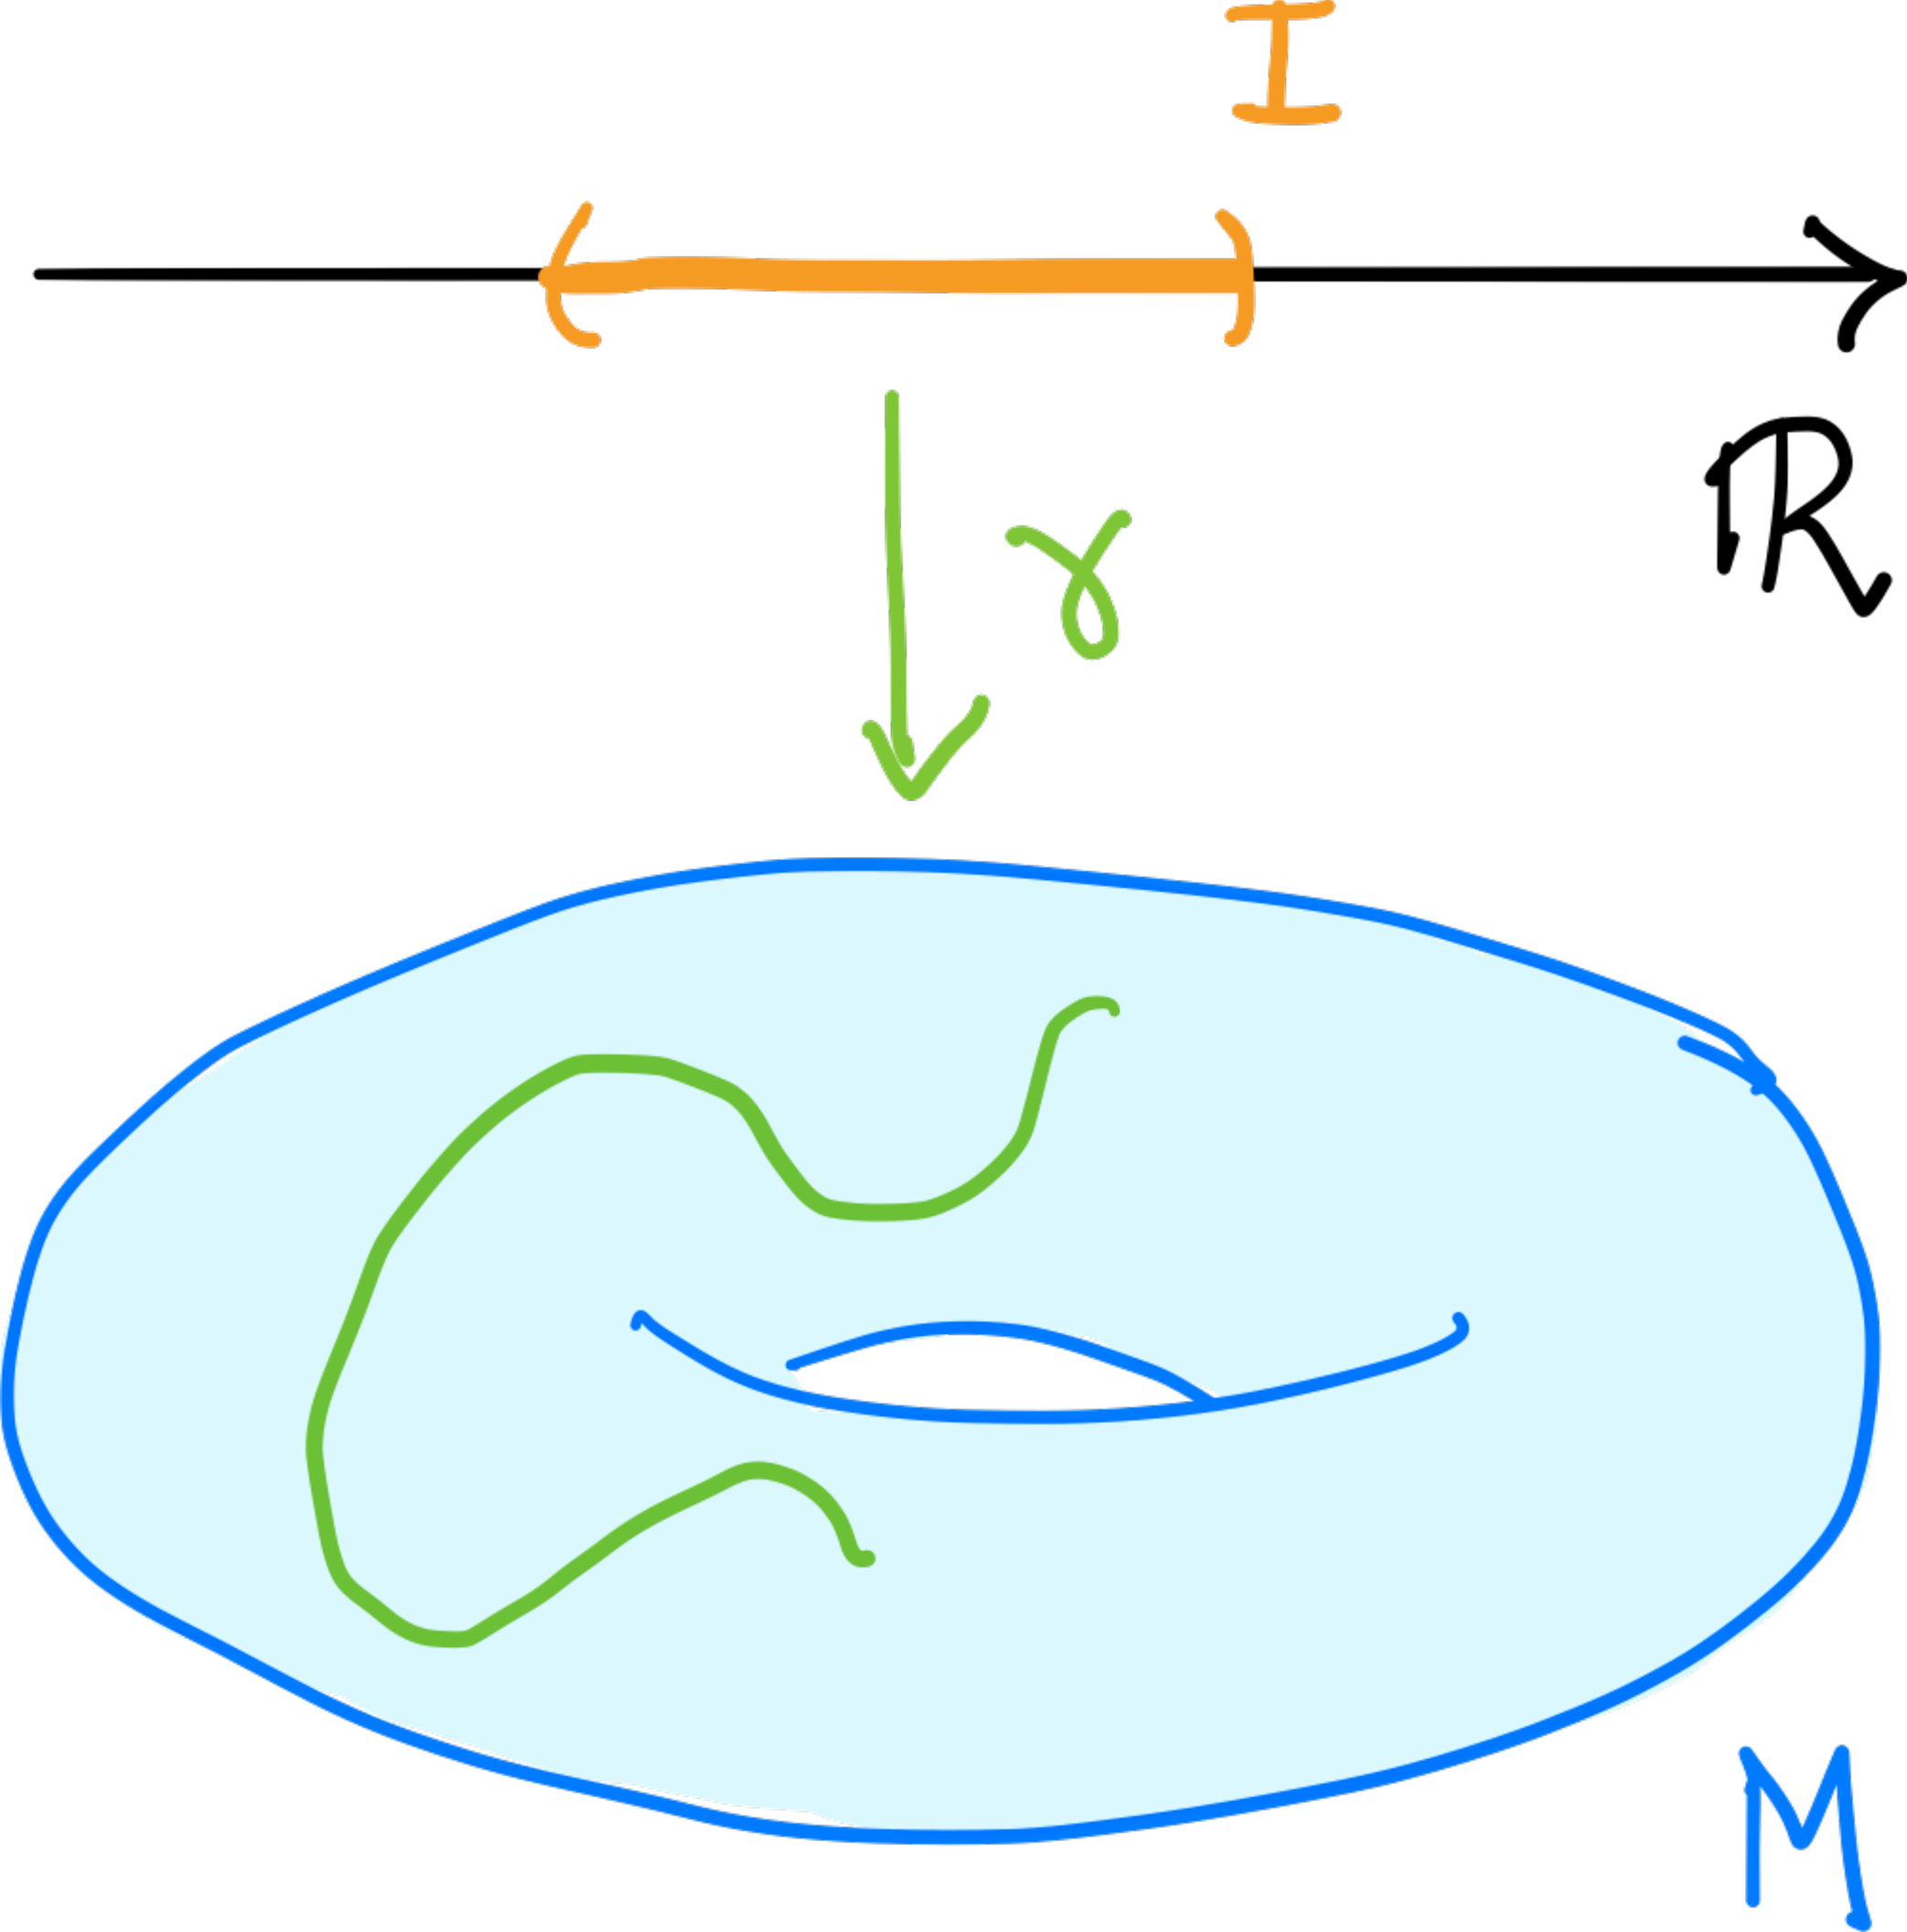
\includegraphics{2_2-curve-on-M.pdf}
\end{marginfigure}

Fix $t\in(a,b)$. 
A priori we have two different ways to define the \emph{velocity vector of $\gamma$ at a time $t$}, that is, an element $\gamma'(t) \in T_{\gamma(t)}M$:
\begin{enumerate}
    \item We can define a derivation on $C^\infty(M)$ at $\gamma(t)$ by setting
    \begin{equation}\label{eq:tg_curve_der}
        \gamma'(t) (f) := (f\circ\gamma)'(t), \quad f\in C^\infty(M).
    \end{equation}
    \begin{exe}
        Show that this is indeed a derivation on $C^\infty(M)$.
    \end{exe}
    \item If we think of $\gamma$ as a smooth map between manifolds, we can define the tangent vector via the differential $d\gamma_t$:
    \begin{equation}\label{eq:tg_curve_diff}
        \gamma'(t):= d\gamma_t\left(\frac{\partial}{\partial t}\Big|_t\right) \in T_{\gamma(t)}M.
    \end{equation}
\end{enumerate}

Do these definition agree?
One way to check is to pick a chart $\phi: U \to \phi(U)$ in a neighborhood of $gamma(t)$, and compare the expressions in local coordinates. Let $(x^i)$ denote the coordinates of $\phi$ and define the curves $\gamma^i := x^i \circ \gamma : I\to\R$.
Let's focus on \eqref{eq:tg_curve_der}. By definition, $\gamma'(t)(x^i) = (x^i\circ\gamma)'(t) = (\gamma^i)'(t)$, therefore by Proposition~\ref{prop:basis_TpM} we get
\begin{equation}\label{eq:tg_curve_vec}
    \gamma'(t) = \sum_{i=1}^m \gamma'(t)(x^i) \frac{\partial}{\partial x^i}\Big|_\gamma(t).
\end{equation}
\begin{exe}
    Show that applying Proposition~\ref{prop:DiffCoords} to \eqref{eq:tg_curve_diff} leads to the same formula as \eqref{eq:tg_curve_vec}.
\end{exe}

\begin{figure*}[htp]
    \centering
    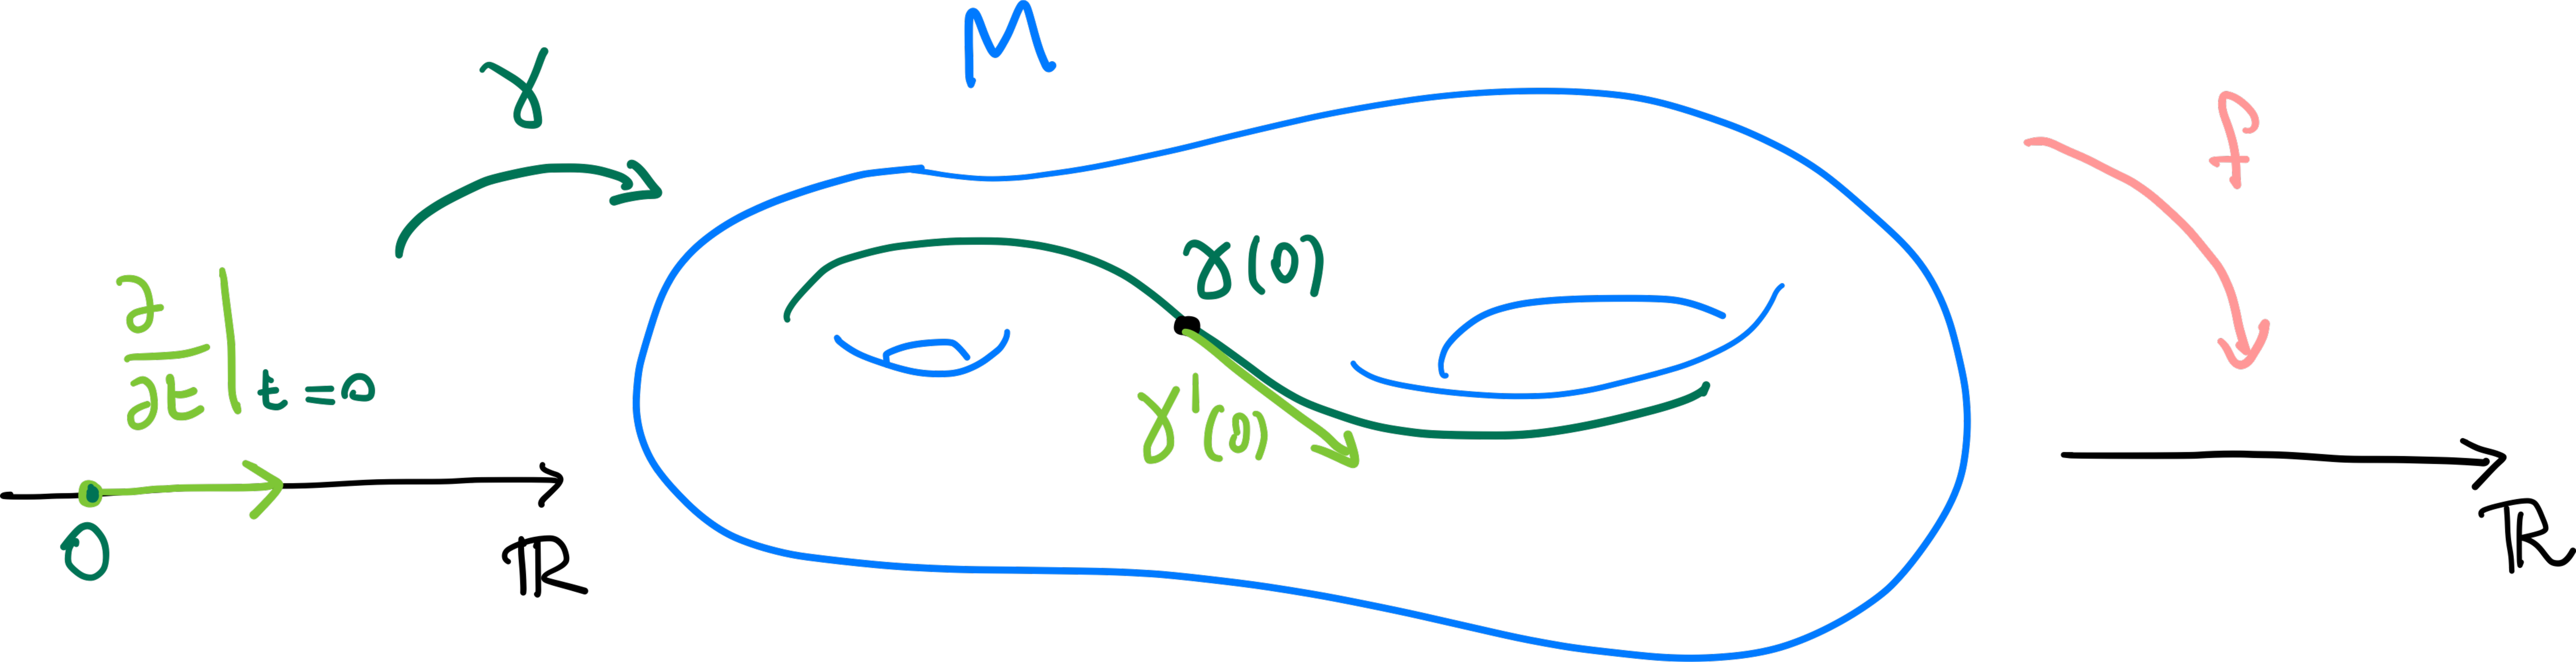
\includegraphics{2_5-v_cur_full.pdf}
    \caption{The velocity of a curve}
    \label{fig:2_5-v_cur_full}
\end{figure*}

But how can this be well defined? Surely, there must be multiple curves with the same speed at a point which differ outside a neighborhood of the point.

\begin{lem}\label{lem:equiv_tg_curves}
    Let $M$ be a smooth manifolds and $\gamma, \delta : (-\epsilon, \epsilon) \to M$ two smooth curves with $\gamma(0) = \delta(0)$. Then, $\gamma'(0) = \delta'(0)$ as elements of $T_{\gamma(0)}M$ if and only if for some (and thus any) chart $\phi:U\to\phi(U)$, $\gamma(0)\in U$, we have $(\phi\circ \gamma)'(0) = (\phi\circ\delta)'(0)$.
\end{lem}
\begin{proof}
    Let $(x^i)$ denote the coordinates of $\phi$. The condition $(\phi\circ \gamma)'(0) = (\phi\circ\delta)'(0)$ is equivalent as stating that $(\gamma^i)'(0) = (\delta^i)'(0)$, where $\gamma^i = x^i\circ\gamma$ and $\delta^i=x^i\circ\delta$. Then, the claim follows from \eqref{eq:tg_curve_vec} and the fact that $\left\{\frac{\partial}{\partial x^i}\big|_{\gamma(0)}\right\}$ is a basis of $T_{\gamma(0)}M$.
\end{proof}

This seems to follow a pattern: until now, all the definitions of tangent vectors where in terms of classes of equivalence.
There is still a potential problem, though. We don't yet know if \emph{every} tangent vector can be written as the velocity vector of a curve.

\begin{thm}
    Let $M$ be a smooth $n$-manifold, let $p\in M$ and let $v\in T_pM$.
    There exists a smooth curve $\gamma: (-\epsilon,\epsilon) \to M$ such that $\gamma'(0) = v$.
\end{thm}
\begin{proof}
    Let $\phi:U\to\phi(U)$ be a chart about $p$ such that $\phi(p)=0$.
    Let $(x^i)$ denote the coordinates of $\phi$, as usual, and assume that
    \begin{equation}
        v = \sum_{i=1}^n a^i \frac{\partial}{\partial x^i}\Big|_p, \qquad a^i \in\R.
    \end{equation}
    For $\epsilon$ small enough, by continuity the vector $(ta^1, \ldots, ta^n) \in \phi(U)$ for all $|t|<\epsilon$. Therefore, the curve
    \begin{equation}
        \gamma: (-\epsilon, \epsilon) \to M, \quad \gamma(t):=\phi^{-1}(ta^1, \ldots, ta^n),
    \end{equation}
    is well-defined, smooth, satisfies $\gamma(0) = p$ and, by \eqref{eq:tg_curve_vec}, $\gamma'(0) = v$.
\end{proof}

\begin{marginfigure}
    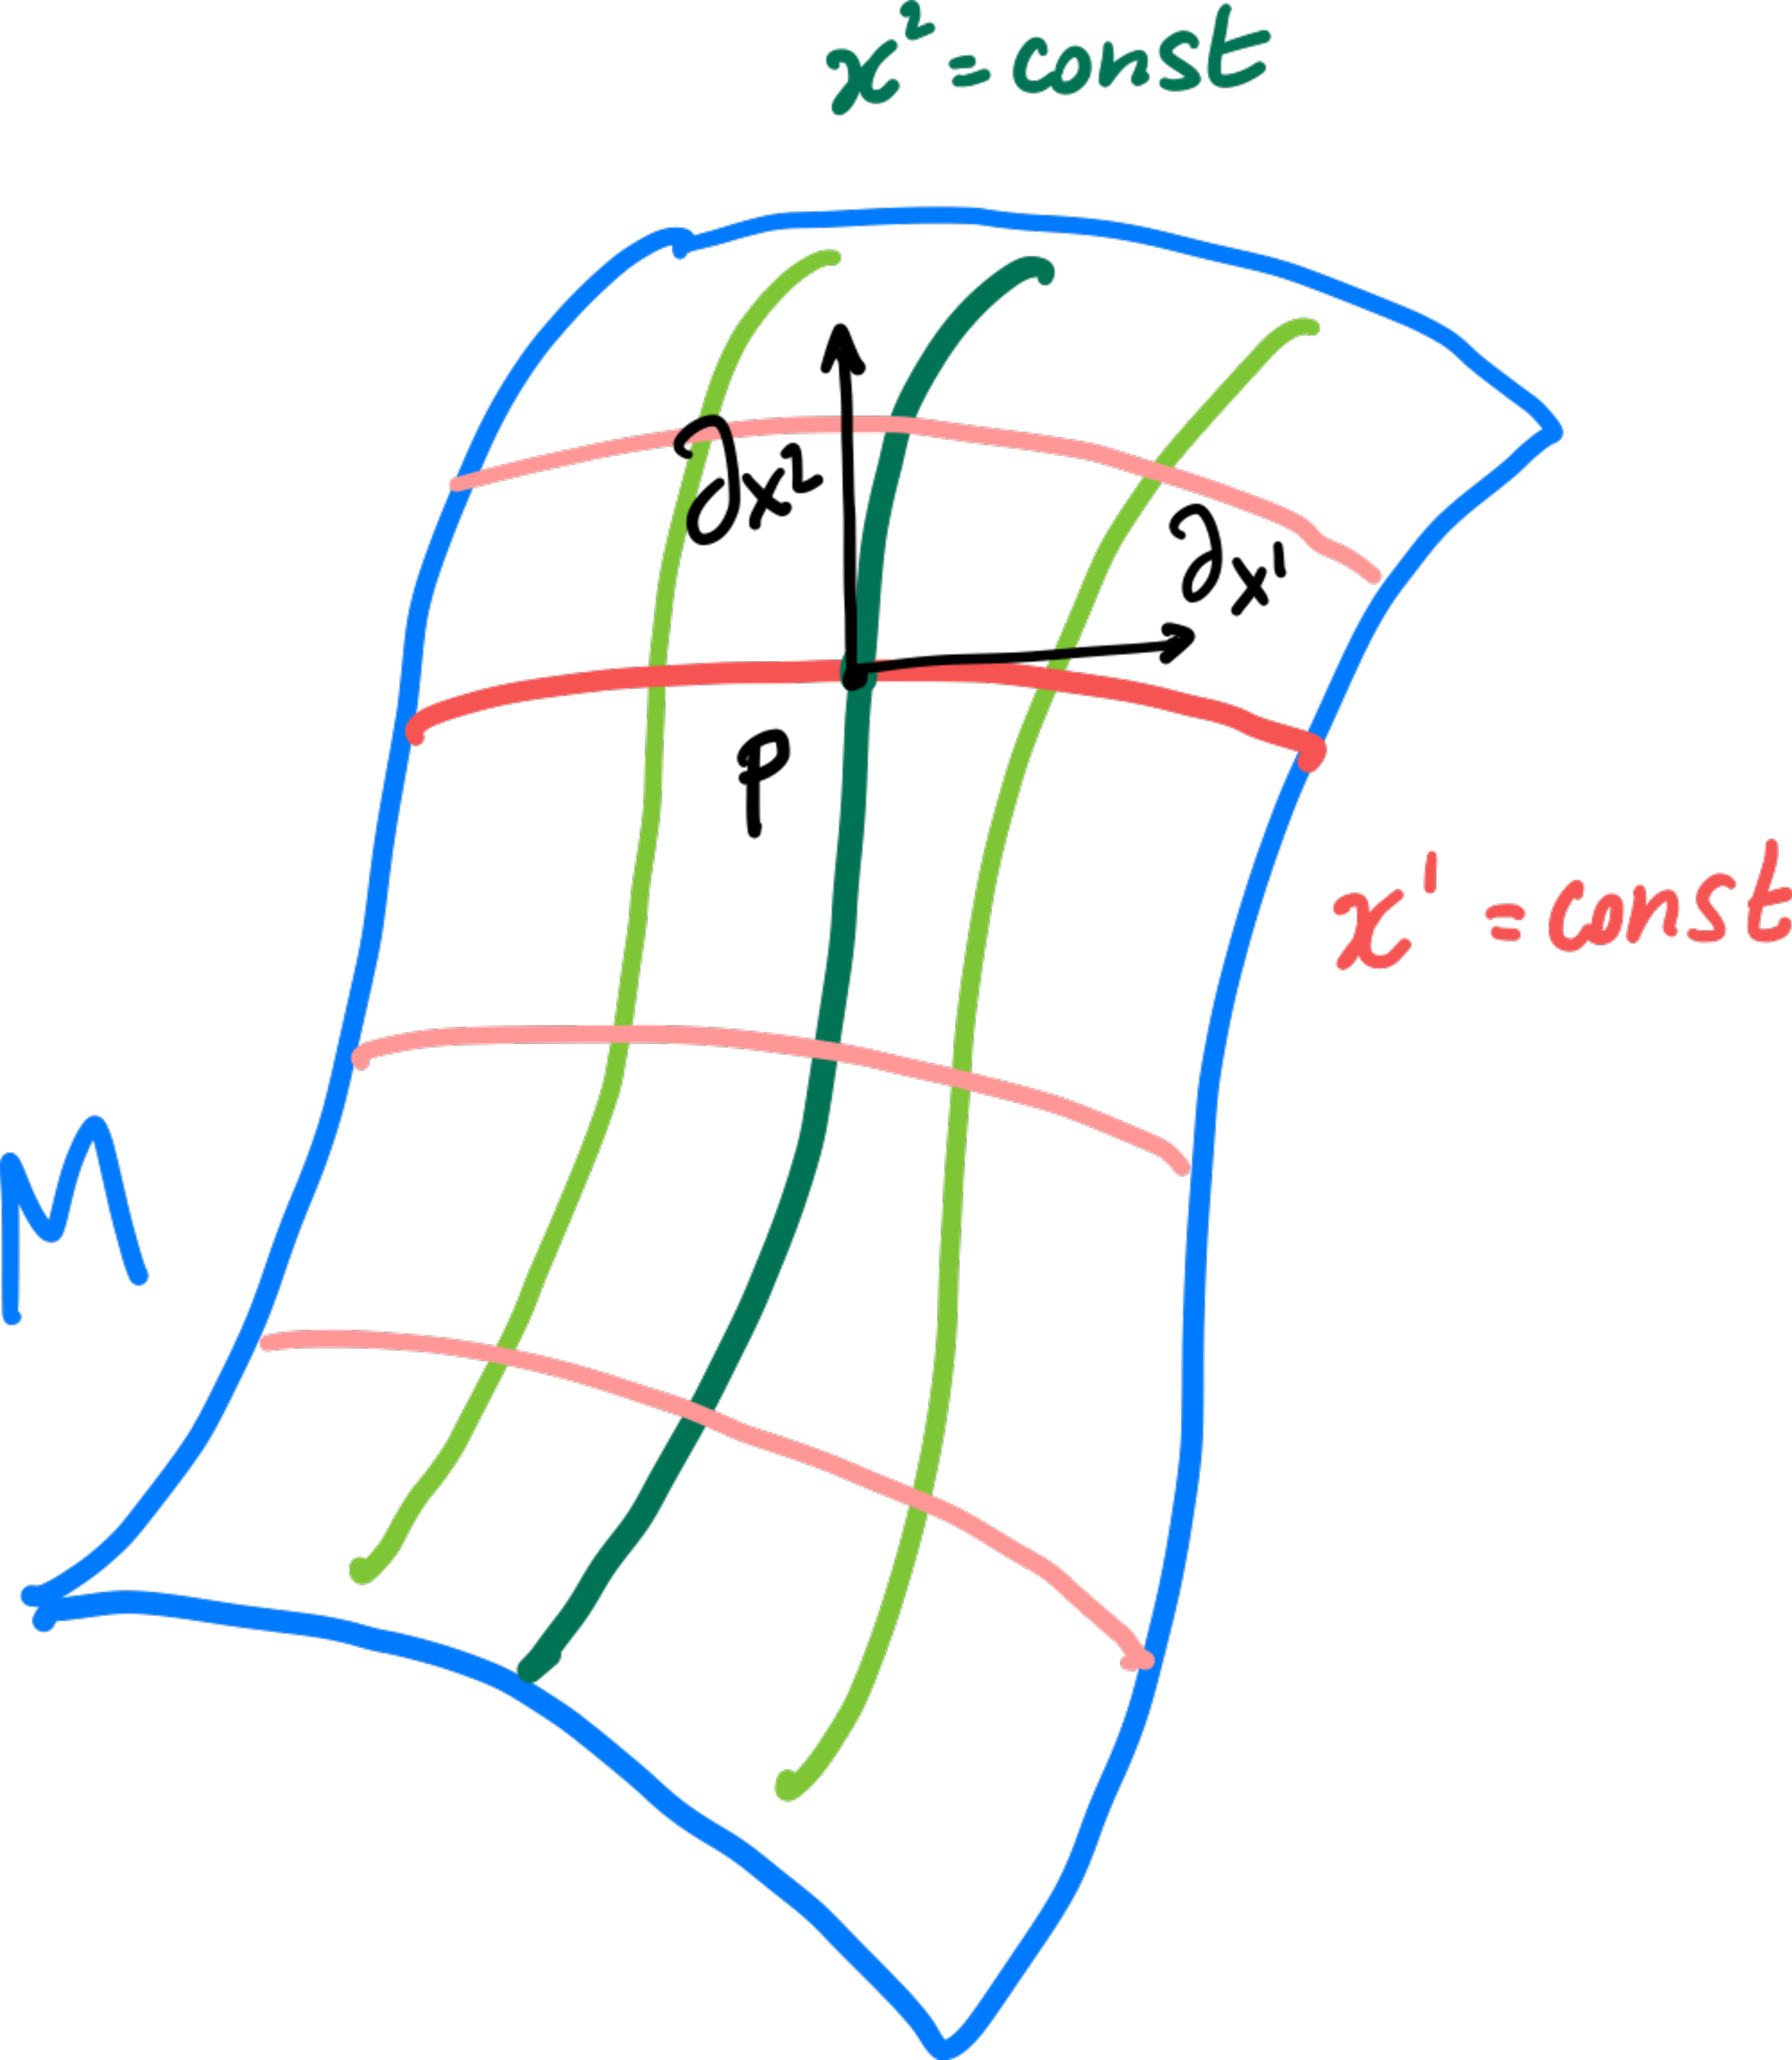
\includegraphics{2_4-v_cur.pdf}
    \caption{With this definition, the coordinate tangent vectors $\partial_{x^i}\in T_p M$ become the tangent vectors defined by the curve \[t \mapsto \phi^{-1}(x^1(p), \ldots, {x^i(p) + t}, \ldots, x^n(p)).\]}
    \label{fig:2_4-v_cur}
\end{marginfigure}
This means that we can actually make an alternative definition of $T_xM$ in terms of tangent to curves:
\begin{quote}
    a tangent vector at $p\in M$ is an equivalence class of smooth curves $\gamma:(-\epsilon, \epsilon)\to M$ such that $\gamma(0)=p$, where $\gamma\sim\delta$ if and only if $(\phi\circ \gamma)'(0) = (\phi\circ\delta)'(0)$ for some chart centered about $p$ (see Lemma~\ref{lem:equiv_tg_curves}).
\end{quote}

In fact, it is possible to start the whole tangent space discussion with the above definition. In that case, you would first need to prove Exercise~\ref{exe:vsstruct} and to endow $T_xM$ with a vector space structure\footnote{To get the analogue result as Proposition~\ref{prop:basis_TpM}}.

To conclude this part, the next proposition shows that velocity vectors behave well under composition with smooth maps and gives us direct, explicit and effective way to compute differentials.

\begin{prop}\label{prop:curves_deriv}
    Let $F:M\to N$ b a smooth map between smooth manifolds and $\gamma:I\to M$ a smooth curve in $M$.
    Then
    \begin{equation}
        d F_{\phi(t)} (\phi'(t)) = (F\circ\gamma)'(t).
    \end{equation}
\end{prop}
\begin{proof}
    We are going to use \eqref{eq:tg_curve_diff} as definition of $\gamma'(t)$.
    Applying the chain rule we obtain:
    \begin{align}
        d F_{\phi(t)} (\phi'(t))
        &= d F_{\phi(t)} \circ d\phi_t \left(\frac{\partial}{\partial t}\Big|_t\right) \\
        &= d (F\circ\gamma)_t \left(\frac{\partial}{\partial t}\Big|_t\right) \\
        &= (F\circ\gamma)'(t).
    \end{align}
\end{proof}

\begin{exe}
    Give an alternative proof of Proposition~\ref{prop:curves_deriv} using \eqref{eq:tg_curve_der} as definition for $\gamma'(t)$.
    Hint: use the definitions to rewrite the formula in different ways.
\end{exe}


\section{The tangent bundle}